\section{Linting and Static Analysis}

% TODO: talk about how my approach is formal methods, not data-driven

% TODO: might be worth talking about soundness and completeness
% Most practical static checkers for JavaScript [3, 2, 1, 4] and other languages [29, 11] take a pragmatic view and favor a relatively low false positive rate over soundness

\textbf{Linting} is the process of analysing source code to identify and report issues related to coding style and potential logical errors.
The term originates from the \texttt{lint} program \cite{johnson_lint_1978}, which examined C source code for bugs, as well as wasteful code patterns that may be legal but error-prone.
The tool was also utilised to enforce portability restrictions which aided users in writing portable code that could be compiled on multiple platforms.
Since the release of \texttt{lint}, many linting tools, known as \textbf{linters}, have been developed for a wide range of programming languages.

Nowadays, many linters can be integrated into \textsc{ide}s, where code analysis performed by the linter is run incrementally in the background.
Any violations found by the linter are displayed directly in the editor as warnings or errors at the relevant locations in the source code.
This brings early, real-time feedback to the programmer, allowing them to address issues as they write code, with minimal interruption to their development workflow.
Linters can also be integrated as part of the code review process, or into continuous integration (\textsc{ci}) pipelines to ensure that code adheres to a set of standards before being merged into the main codebase.

Although the traditional definition for linting is concerned only with \emph{detecting} issues in code, modern linters have broadened their scope significantly.
In addition to detecting issues, many linters provide \emph{auto-fix} capabilities to correct issues by automatically rewriting the offending code snippets.
This feature is often integrated into \textsc{ide}s as well: the popular Language Server Protocol for defining \textsc{ide} features enables these auto-fix features via \emph{code actions} \cite{gunasinghe_lsp_2022}.
When a section of code is highlighted by a linter warning, a user can apply a code action to automatically fix the issue with a single click.

Linters and related static analysis tools are increasingly becoming more important in modern software development, as modern code continues to become more complex and difficult to reason about.
Industry leaders, such as Google \cite{sadowski_analysis-google_2018} and Meta/Facebook \cite{calcagno_moving-facebook_2015}, have embraced these tools as integral components of their software development workflows.
The use of automated tools to detect potential issues is not only faster but in some cases more effective than human review, saving developer time and reducing error rates in the development process.

\subsection{Types of Issues Detected by Linters}

Many linters are configurable with a set of rules, which specify the categories of issues that the linter should detect.
These rules can be enabled or disabled by users, allowing them to customise the linter to their needs.
Rules are usually grouped by purpose: some rules are concerned with simply improving code style, while others are concerned with detecting suspicious code patterns indicative of potential bugs.

\subsubsection{Style checks and code quality}

Linters can suggest opportunities to improve code by utilising language features in a more idiomatic manner.
Snippets of code that violate these stylistic rules are not necessarily incorrect, but should be fixed as they may be harder to read or maintain in the long term.
Furthermore, many idiomatic practices exist to avoid common pitfalls that could lead to unintended behaviour.
By highlighting good practices, linters can help users avoid these common mistakes that may cause bugs.
For example, \emph{ESLint}\footnote{\url{https://eslint.org/docs/latest/rules/}}, one of the most popular JavaScript linters, warns against common JavaScript pitfalls such as using the regular equality operator \texttt{==} instead of its type-safe alternative \texttt{===}.

A well-designed linter can help programmers learn about useful language constructs by suggesting them in the context of their code, aiding them in adhering to best practices and common style conventions.
This category of rules is therefore especially helpful as an educational tool for new users of a language, who may be unaware of these idioms.
For example, the \emph{Clippy}\footnote{\url{https://doc.rust-lang.org/clippy/}} linter for Rust \cite{li_clippy_2023} categorises a collection of rules as \texttt{clippy::complexity} rules to detect code that does something simple in a complex way and suggests a simpler alternative.
\Cref{fig:hlint-example} provides an example of a similar rule in Haskell, from the \textit{HLint}\footnote{\url{https://hackage.haskell.org/package/hlint}} linter.
The rule suggests to rewrite the function into an equivalent but more concise form via $\eta$-reduction, presented to the user as a code action that can be applied automatically.

\begin{figure}[htbp]
  \vspace{3ex}
  \centering
  \begin{subfigure}{0.45\textwidth}
    \centering
    \begin{minted}[frame=single]{haskell}
      foo xs = map (+1) xs
    \end{minted}
    \caption{A Haskell function \texttt{foo}, which can be made more concise using $\eta$-reduction.}
  \end{subfigure}
  \hfill
  \begin{subfigure}{0.45\textwidth}
    \centering
    \begin{minted}[frame=single,escapeinside=||]{text}
      Eta reduce
      Found:
        foo xs = map (+ 1) xs
      Why not:
        foo = map (+ 1)
      |\textcolor{gray}{hlint(refact:Eta reduce)}|
    \end{minted}
    \caption{The linter warning shown for \texttt{foo}.}
  \end{subfigure}
  \caption{An example of a warning from the Haskell linter \texttt{hlint}, suggesting a fix that a user can choose to automatically apply.}
  \label{fig:hlint-example}
\end{figure}

\paragraph{Domain-specific idioms}
A library or especially an embedded \textsc{dsl} may require a particular style of usage that is different from the host language \cite{hora_domain_2012}.
The majority of linters are designed for general-purpose application domains, so they are unlikely to detect issues specific to a more specialised domain.
Therefore, linters may be developed for specific libraries or \textsc{dsl}s, with their own set of domain-specific rules.
In this case, the accompanying linter can benefit users and improve developer productivity in a similar manner to general-purpose linters: common misuses can be detected and sometimes automatically fixed, and users can be directed to relevant documentation to learn more about correct usage.
For instance, the \emph{xUnit.net} testing framework for C\# is accompanied by the \texttt{xunit.analyzers}\footnote{\url{https://github.com/xunit/xunit.analyzers}} package which provides linting rules to enforce best practices specific to \emph{xUnit}.

\subsubsection{Code smells and opportunities for refactoring}

Code refactoring is a well-established practice in software development.
In his influential book \emph{Refactoring: Improving the Design of Existing Code} \cite{fowler_refactoring_2018}, Fowler defines \textbf{refactoring} as ``the process of changing a software system in such a way that it does not alter the external behaviour of the code yet improves its internal structure''.
Refactoring may be employed to eliminate \textbf{code smells}, which are surface indications that could indicate deeper problems in the system.
Code smells are not necessarily problematic on their own, however, they may lead to issues such as bugs or poor maintainability if left unchecked.
They are conceptually similar to the stylistic issues mentioned earlier, however they may encompass higher-level structural and design-based problems that are not easily fixed by simple stylistic changes.
Examples of code smells include duplicated code, which can be hard to update without introducing bugs, and long methods, which can be difficult to understand and maintain.
Therefore, it is often productive to refactor code to eliminate code smells, even if the code is still correct and functional.

Certain linting rules can aid in the refactoring process by broadly identifying code smells and candidate areas for refactoring, suggesting appropriate actions that the user can take.
As an example, a linter may detect a fragment of code that is repeated in multiple places: this is a code smell, as discussed previously.
The linter may then suggest a code action to automatically apply an \emph{Extract Method} \cite{fowler_refactoring_2018} refactoring to avoid code duplication: \cref{fig:extract-function-intellij} demonstrates how this automatic refactoring process can be performed in the IntelliJ IDEA\footnote{\url{https://www.jetbrains.com/idea/}} \textsc{ide}.

\begin{figure}[htbp]
  \centering
  \begin{subfigure}{\textwidth}
    \centering
    \begin{minted}[frame=single,highlightlines={4-5},linenos]{scala}
      object Main {
        def main(args: Array[String]): Unit = {
          val bankDetails = getBankDetails()
          println(s"Account name: ${bankDetails.name}")
          println(s"Account balance: ${bankDetails.balance}")
        }
      }
    \end{minted}
    \caption{A snippet of Scala code. A user may wish to extract the highlighted lines into a separate function.}
    \label{fig:extract-function-intellij-before}
  \end{subfigure}
  \begin{subfigure}{\textwidth}
    \centering
    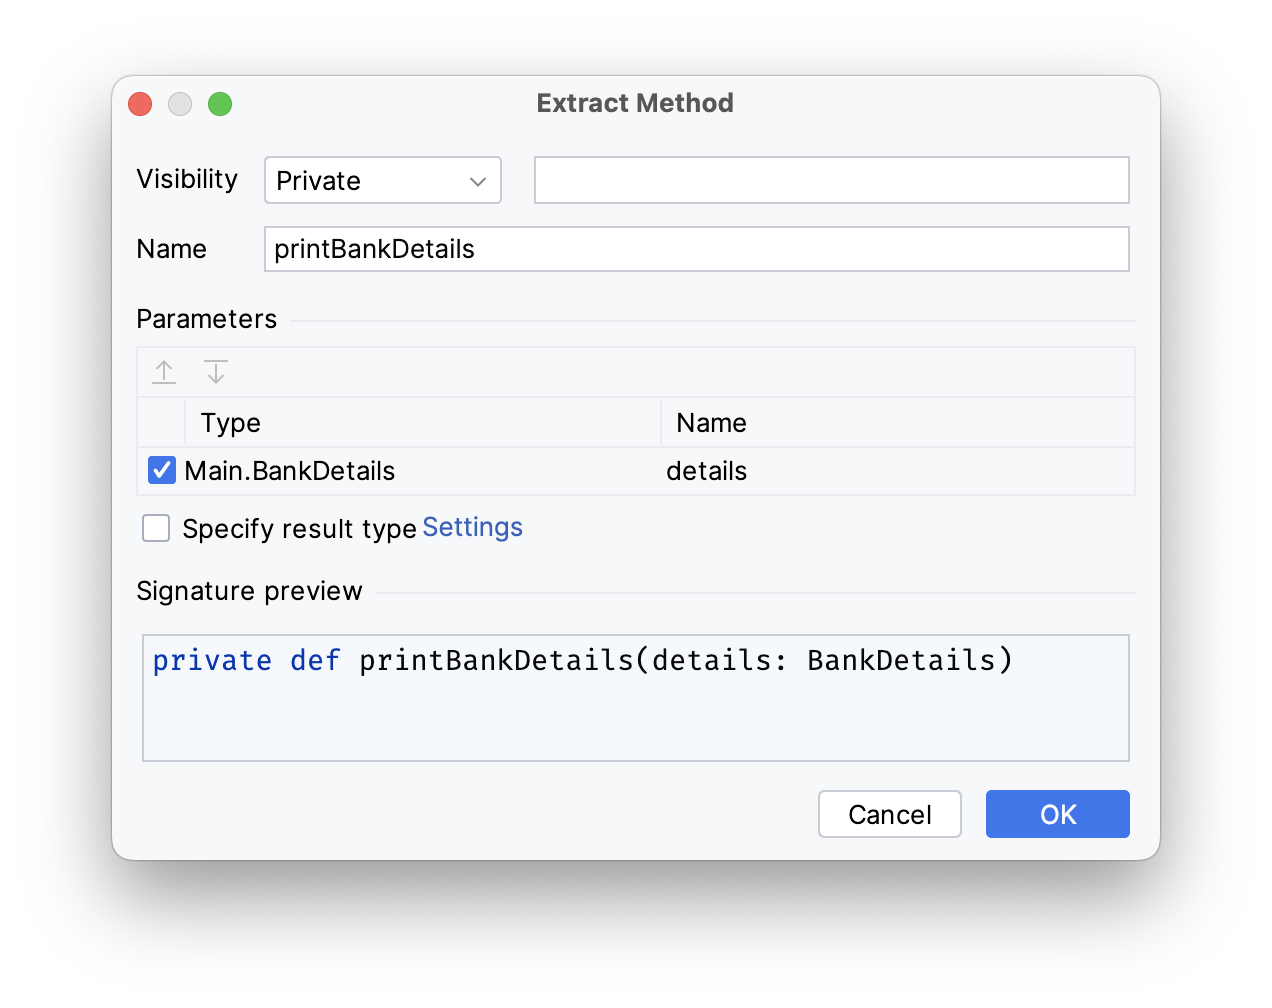
\includegraphics[width=0.75\textwidth]{src/background/extract-function-intellij.png}
    \caption{When a user selects the highlighted lines from \cref{fig:extract-function-intellij-before} in IntelliJ IDEA, choosing the \emph{Extract Method} refactoring will open this dialogue to preview changes before applying them.}
    \label{fig:extract-function-intellij-dialogue}
  \end{subfigure}
  \begin{subfigure}{\textwidth}
    \vspace{3ex} % TODO: ew
    \centering
    \begin{minted}[frame=single,highlightlines={4,7-10},linenos]{scala}
      object Main {
        def main(args: Array[String]): Unit = {
          val bankDetails = getBankDetails()
          printBankDetails(bankDetails)
        }

        private def printBankDetails(details: BankDetails): Unit = {
          println(s"Account name: ${details.name}")
          println(s"Account balance: ${details.balance}")
        }
      }
    \end{minted}
    \caption{The result of applying the \emph{Extract Method} refactoring using the chosen parameters in \cref{fig:extract-function-intellij-dialogue}.}
  \end{subfigure}
  \caption{An example of the \emph{Extract Method} refactoring in IntelliJ IDEA.}
  \label{fig:extract-function-intellij}
\end{figure}

\subsubsection{Possible bugs or errors}

Linters may also directly attempt to detect more serious issues in code, such as possible logic errors.
This can be helpful for even experienced users to avoid common pitfalls.
For example, \emph{Clippy} has \texttt{clippy::suspicious} and \texttt{clippy::correctness} rule categories to identify code that is very likely to be incorrect or useless.
\emph{ESLint} provides several rules to warn against code patterns that are likely to cause runtime errors, such as re-assigning a \texttt{const} variable.

Again, linters may attempt to provide auto-fixes for these issues where possible.
However, these issues are usually more complex, which may limit the effectiveness or usefulness of auto-fixes: in the case of a suspicious code pattern, the programmer's intent may not be clear, causing the linter to suggest a fix that does not align with the user's expectations.

\subsection{Implementing Linters}

\TODO{This is the old static analysis section - rework this}

The vast majority of linters are implemented using static program analysis, analysing source code to extract information about its behaviour without executing the program itself. 
This is in contrast to dynamic analysis, which is performed on programs as they are run.
Although dynamic analysis can yield more precise results as it observes the actual runtime behaviour of the program, it is also more heavyweight as a result.

Given their need to be scalable and efficient enough to handle entire codebases, linters are designed to be fast and lightweight.
In most practical cases, therefore, dynamic analysis is too slow and resource-intensive to be used for the purpose of linting.
However, dynamic languages such as JavaScript present challenges for static analysis due to their dynamic runtime nature.
This has led to the exploration of linters that incorporate dynamic analysis techniques to identify issues that static methods cannot detect \cite{gong_dlint_2015}.
Despite these developments, state-of-the-art JavaScript linters utilised in industry, such as \emph{ESLint}, still solely rely on static analysis.

\TODO{
* parsley is a scala library
* scala is a static language, strongly typed
* this section will therefore focus on the traditional static analysis approach, since dynamic analysis is not as relevant here

https://scalacenter.github.io/scalafix/docs/users/related-projects.html
Lint on compile vs lint after compile?
}

\subsubsection{AST stuff}

\TODO{
* how does HLint work? seems like its sometimes prone to false positives
}

Static analysis tools can reason about how to safely refactor code in an automated manner, performing refactorings as source-to-source transformations.
These transformations may be implemented as simple text-based replacements or more robust rewrite rules that operate on the abstract syntax tree (\textsc{ast}) of the source code.


% TODO: justification why we don't use dynamic analysis? linters - static, lightweight

These tools can perform a variety of tasks, ranging from detecting possible bugs \cite{johnson_lint_1978,hovemeyer_finding-bugs_2004} to formal software verification of program properties \cite{blanchet_static-analyzer_2003}.

\section{Static Analysis for Scala}

\TODO{DSL linting is hard but luckily Parsley is an eDSL so we can just use Scala metaprogramming utilities}

\subsection{Choice of Tooling}
The goal of \texttt{parsley-garnish} is to provide linting and refactoring capabilities for the \texttt{parsley} parser combinator library.
Since \texttt{parsley} is a Scala library, this project must be implemented using a tool capable of statically analysing Scala code.
This section will therefore discuss and evaluate the choices available for implementing \texttt{parsley-garnish}.

\paragraph{Scala compiler plugins}
The most powerful approach would be to implement \texttt{parsley-garnish} as a compiler plugin \cite{pickering_plugins_2019}.
Using the low-level compiler \textsc{api}, it is possible to perform arbitrary code transformations at any step of the compilation process.
Compiler plugins therefore offer full freedom to extend the Scala compiler with extra functionality, such as extra passes for code analysis and emitting lint warnings as diagnostics or even compiler errors.

However, this approach has several drawbacks.
Firstly, compiler plugins are tightly coupled with the compiler itself, and therefore not portable across major compiler versions.
% https://github.com/mattmoore/scala-compiler-plugins is a good reference, in case I need to revisit this
For instance, plugins written for the Scala 3 compiler, known as \texttt{dotty}, are completely incompatible with Scala 2 plugins \cite{lampepfl_changes_2022}.
Additionally, developing compiler plugins requires a deep understanding of arcane and poorly documented compiler internals.
Exposing the full compiler \textsc{api} permits unsafe operations that may violate undocumented invariants assumed by the compiler, leading to exceptions during compilation or even malformed bytecode \cite{sherwany_refactoring_2015}.
The lack of higher-level abstractions also makes it difficult to implement even trivial tasks such as renaming a field.

For these reasons, it would be preferable to explore other tools that may use compiler plugins themselves but provide a higher-level interface for implementing code analysis and transformations.

\paragraph{Scalameta}
\textit{Scalameta}\footnote{\url{https://scalameta.org/}} is a metaprogramming framework for Scala that provides a unified interface for performing common metaprogramming tasks.
It provides a high-level syntactic \textsc{api} for transforming and pretty-printing Scala source code, as well as a semantic \textsc{api} providing access to semantic information such as type inference and name resolution.
\TODO{make this clearer about the unification of runtime and compile-time metaprogramming? scalameta does more than scala-reflect}
Scalameta is the successor of the earlier \texttt{scala.reflect} metaprogramming framework, which parsed source code into lossy trees that discarded syntactic information such as comments and whitespace \cite{burmako_scalameta_2017}.
\TODO{this is called hygiene right?}
On the other hand, Scalameta trees are lossless and preserve all syntactic details, a key feature that allows code transformations and refactorings to preserve formatting details.

Scalameta's semantic \textsc{api} is powered by \textit{SemanticDB}, a compiler-agnostic data model for semantic information in Scala programs.
This allows Scalameta to extract semantic information via compiler plugins that emit data in the SemanticDB format.
Thus, Scalameta can work with any compiler that supports SemanticDB, rather than being tied to a specific compiler implementation.

Since Scalameta provides a high-level interface for manipulating syntactic and semantic information, it is a promising choice for this project.
Being able to access semantic information is especially helpful for implementing more complex code analyses.
However, Scalameta's primary focus is on providing a general metaprogramming framework and therefore lacks \textsc{api} support specifically for implementing linting and refactoring rules.
For example, the Scalameta tree transformation utilities do not preserve formatting details when pretty-printed, despite the underlying trees containing this information.

\paragraph{Scalafix}
% Scalafix is fundamentally a general-purpose code linter and code rewriter
\textit{Scalafix}\footnote{\url{https://scalacenter.github.io/scalafix/}} is a refactoring and linting tool built on top of Scalameta.
It specifically provides an \textsc{api} for implementing fine-grained code transformations that preserve comments and formatting details.
Scalafix provides a framework for implementing linting rules to emit warnings, as well as rewrite rules to perform automated code transformations \cite{geirsson_catch_2017}.
Since it is built on Scalameta, a major advantage of Scalafix is that it is also compiler-agnostic and could be integrated into any \textsc{ide} if a plugin is developed for it.

Originally, Scalafix was designed to help automate the process of migrating code from Scala 2 to 3, which involved many breaking changes to the language \cite{geirsson_scalafix_2016}.
However, Scalafix has since evolved into a general-purpose tool for implementing code transformations and analyses, utilising the powerful syntactic and semantic \textsc{api}s provided by Scalameta.
Scalafix rules can be either syntactic or semantic, depending on whether they require semantic information to perform their analysis.
Syntactic rules are faster to run, since they operate purely on the \textsc{ast} without requiring compilation to extract semantic information, but are more limited in the accuracy of analyses they can perform.

Scalafix is growing to become the de-facto modern successor to earlier refactoring tools such as Abide\footnote{\url{https://contributors.scala-lang.org/t/whats-the-status-of-abide/}} and \texttt{scala-refactoring}\footnote{\url{https://github.com/scala-ide/scala-refactoring}}.
\texttt{scala-refactoring} used \texttt{scala.reflect} to implement code transformations, with much extra work utilising the Scala Presentation Compiler \textsc{ast} to preserve formatting details lost by \texttt{scala.reflect}.
As a result, maintaining the library became difficult and the project was abandoned in favour of a clean implementation using Scalameta, which was designed in part to address the shortcomings of \texttt{scala.reflect}.

A drawback of Scalafix is that it is primarily a command-line tool, and therefore by default does not provide a user-friendly interface for interactive usage. % TODO: expand this: cite jaglin's talk, especially since metals backend also uses semanticdb
However, this can rectified in the future by integrating Scalafix into the Metals \textsc{lsp} server for Scala, which would allow it to be integrated into any \textsc{ide} that supports the LSP.

Overall, Scalafix emerges as the most favorable choice for implementing \texttt{parsley-garnish}.
It provides high-level \textsc{api}s specifically for implementing linting and rewrite rules without necessitating extensive knowledge of compiler internals.
Scalafix is also being actively developed and maintained, with good basic documentation and a growing number of examples of usage in the wild.

\paragraph{Other tools considered}
The main alternate contender to Scalafix is the IntelliJ Scala Plugin\footnote{\url{https://github.com/JetBrains/intellij-scala}}.
However, while the plugin offers superior interactive usage within the IntelliJ IDEA \textsc{ide}, it is tied to the IntelliJ Scala compiler and therefore not portable across other compilers.
To maintain flexibility and not tie \texttt{parsley-garnish} to a particular compiler or code editor, Scalafix is a preferable option.
Furthermore, documentation is less clear on how to write a Scala plugin for IntelliJ compared to the Scalafix documentation.

WartRemover\footnote{\url{https://www.wartremover.org/}} is a linter implemented as a compiler plugin, with support for writing custom rules.
However, it only can emit warnings or errors and does not support auto-fixes, making it less suitable for \texttt{parsley-garnish}'s goals.

ScalaStyle\footnote{\url{http://www.scalastyle.org/}} is primarily a style checker which also supports custom rules.
However, it is only able to perform syntactic analyses and does not have access to semantic information, restricting the types of analyses it can perform.

% TODO: maybe a section introducing ScalaFix and how it works? or is that too much detail?
% TODO: maybe a figure to show an example of a ScalaFix rewrite rule?

% TODO: comparison with clippy (https://doc.rust-lang.org/clippy/development/lint_passes.html) and/or roslyn (https://learn.microsoft.com/en-us/dotnet/csharp/roslyn-sdk/; https://learning.oreilly.com/library/view/roslyn-cookbook/9781787286832/)

\subsection{Scalafix}
Two categories of scalafix rules: syntactic and semantic.~\cite{scalacenter_scalafix_2024}
Syntactic rules don't require compilation, so they are easier to run. However this also means they can only do limited code analysis, as they don't have access to compiler information such as symbols and types.
Semantic rules, on the other hand, require compilation and are therefore slower and more complicated to run. However, they are able to perform more advanced code analysis since they have access to the compiler information that syntactic rules lack access to.

Scalafix rules can act like traditional linters, solely emitting diagnostics for issues in the code.
They can also apply rewrites to transform code as an automatic fix to the issue.

\subsubsection{Internals}
Scalafix parses each source file to generate AST once, each rule gets fed this AST later.

The compiler information that semantic rules use is provided by the \texttt{semanticdb-scalac} compiler plugin.
This is injected immediately after the \texttt{typer} phase of the \texttt{scalac} Scala compiler, allowing it to harvest and dump semantic information in SemanticDB format.~\cite{scalameta_semanticdb_guide_2023}
Basically a stripped-down version of \textsc{tast}y (Typed Abstract Syntax Trees)\footnote{\url{https://docs.scala-lang.org/scala3/guides/tasty-overview.html}} but for both scala 2 and 3.
Scalafix then presents a seamless API to implement semantic rules, allowing users to inspect an AST node and any semantic information associated with it.

\subsubsection{Implementing Rules}
Scalafix rules are metaprograms -- they manipulate Scala programs.
This is achieved by a generic traversal through the AST, represented as a SemanticDB Tree datatype.
Generate side effects with Patches, which represent either lint diagnostics or code rewrites.
Rewrite Patches are pure strings, so this isn't the safest way to do things as there are no guarantees that the output is a well-formed program.
This shortcoming can be somewhat mitigated by instead representing rewrites as Trees, and only converting them to strings right before applying the Patch. % TODO: further discussion somewhere about Squid quasiquotes? 
Patches generated by rules get collected, and applied in a batch rewrite at the end

What semantic information is available to the user?
Trees may have symbol information affixed to them: global symbols are guaranteed to be unique across all documents processed by semanticDB, but local symbols are not~\cite{scalameta_semanticdb_spec_2023}.
This is not necessarily an issue for us, because scalafix rules are only applied per-file anyways so everything should be unique within the file.
Scalafix API provides \scala{SymbolMatcher} to easily create predicates to match specific symbols during traversal of the \textsc{ast}.

\scala{SymbolInformation} also provides other metadata, especially useful is its type signature provided from the compiler's type-checking stage.
A tree may also contains \scala{synthetics} data, granting access to implicit parameter application, and surface syntactic sugar added by compiler.
\scala{SemanticDocument.diagnostics} checks contextual (contextualised = we know which parts of the code the warnings is for) compiler warnings.
